\chapter{Jednorozměrná lineární regrese}
Předpokládejme, že sledujeme dvě veličiny $ x $ a~$ y $ mezi~kterými existuje lineární závislost

$$
	y = \beta_{0} + \beta_{1} x,\quad \text{kde } \beta_{0}, \beta_{1} \text{ neznáme.}
$$

Provede se~experiment a~zjistí se~hodnoty dvojic ($ x , y $). Často se~stává, že $ x $ je změřeno prakticky zcela přesně.

\begin{remark}
 To nastává například v~případě, kdy se~$ x $ nastavuje na~předem dané úrovni a~následně se~k~němu změří odpovídající $ y $.
\end{remark}
 
Oproti tomu u~$ y $ obvykle předpokládáme měření s~chybou. Chyba může být náhodná a~proto i~$ y $ budeme chápat jako náhodnou veličinu, kterou budeme značit $ Y $. Pro~dvojice $ (x_{1}, Y_{1}), \dots ,( x_{n}, Y_{n} )$ se~zavádí model

$$
	Y_{i} = \beta_{0} + \beta_{1} x_{i} + e_{i} \quad (*) \quad i= 1, \dots ,n.
$$

Jednotlivé proměnné se~pak nazývají následovně

\begin{itemize}
  \item $ Y_{i} $ -- vysvětlovaná (závislá) proměnná
  \item $ x_{i} $ -- vysvětlující (nezávislá) proměnná, \textit{popřípadě prediktor nebo regresor}
  \item $ \beta_{0},\beta_{1} $ -- neznámé regresní parametry
  \item $ e_{i} $ -- náhodný šum, (náhodná chyba)
\end{itemize}

Budeme předpokládat, že $ e_{i} $ jsou nezávislé (někdy bude dokonce stačit, aby byly nekorelované) a~$ e_{i} \sim (0,\sigma ^{2}) $. A~tedy splňuje $ \E [ e_{i} ]  = 0 $ , $ \D [ e_{i} ] = \sigma ^{2} $ pro~$ \forall i~$ (homoskedasticita).

Měřením získáme data $ (x_{1}, y_{1}), \dots ,( x_{n}, y_{n} )$ a~cílem statistické analýzy je určit, zda model ($*$) schopen popsat pozorovanou variabilitu u~$ y $. 

\textbf{První krok }

Odhadneme neznámé parametry $ \beta_{0}, \beta_{1}, \sigma^{2} $. Proložíme data přímkou ve~tvaru
$$
	\widehat{y}(x) = \wbeta_{0} + \wbeta_{1} x 
$$
a porovnáme $ y_{i} $ -- \textit{naměřená data} a~$ \widehat{y}(x_{i}) $ -- \textit{predikovaná hodnota lineární regrese} pro~$ \forall i~$. To nám umožňuje posoudit adekvátnost modelu.

Pro proložení dat přímkou existuje několik způsobů. Zásadní ovšem bude znalost rozdělení $ e_{i} $ a~tady i~$ Y_{i} $ i~když apriori není zřejmé proč znát rozdělení a~ne $ \beta_{0}, \beta_{1} $.

Zde máme následující možnosti:

\begin{enumerate}
  \item Odhadnout $ \beta_{0} , \beta_{1} $ pomocí metody nezávisející na~rozdělení chyb
  \item Udělat věrohodnostní předpoklad o~rozdělení chyb, odhadnout $ \beta_{0} , \beta_{1} $ a~následně ověřit předpoklad
\end{enumerate}


\begin{remark}
 Speciální důležitý případ je $ e_{i} \sim \text{N}(0,\sigma^{2}) $ který při~MLE odhadu $ \beta_{0}, \beta_{1} $ vede na~metodu nejmenších čtverců, která může být použita bez~ohledu na~rozdělení chyb.
\end{remark}

\section{Odhady parametrů}
\subsection*{Data s předpokladem normality dat}
Předpokládáme, že $ e_{1}, \dots , e_{n} ~iid~ \text{N}(0,\sigma^{2}) $. To znamená, že $ Y_{i} \sim \text{N}(\beta_{0} + \beta_{1} x_{i},\sigma^{2}) $ a~jednotlivé $ Y_{1}, \dots , Y_{n} $ jsou nezávislé.

\textbf{MLE odhady}

Věrohodnostní funkce je ve~tvaru

$$
\begin{aligned}
	L = L ( \beta_{0} , \beta_{1} , \sigma^{2} ) = \left( \frac{1}{ \sqrt{ 2 \pi \sigma^{2} }} \right) ^{n} \text{exp} \left( - \frac{1}{2 \sigma^{2} } \sum_{i = 1}^{n}( y_{i} -  \beta_{0}  - \beta_{1} x_{i} )^{2} \right) \\
l = \text{ln} L = -\frac{n}{2} \text{ln} ( 2 \pi ) -\frac{n}{2} \text{ln} (\sigma^{2} ) - \frac{1}{2 \sigma^{2} } \sum_{i = 1}^{n}( y_{i} -  \beta_{0}  - \beta_{1} x_{i})^{2}
\end{aligned}
$$

pro pevné $ \sigma^{2} > 0 $ je maximalizace $ l $ ekvivalentní s~minimalizováním $ S~$, kde

$$
S = S~( \beta_{0} , \beta_{1} ) = \sum_{i = 1}^{n}( y_{i} -  \beta_{0}  - \beta_{1} x_{i})^{2}.
$$

Proto tuto metodu někdy nazýváme metodou nejmenších čtverců.

$$
\begin{aligned}
\frac{\partial S}{\partial \beta_{0}} = - 2 \sum_{i = 1}^{n}( y_{i} -  \beta_{0}  - \beta_{1} x_{i}) = 0 , \\
\frac{\partial S}{\partial \beta_{1}} = - 2 \sum_{i = 1}^{n}( y_{i} -  \beta_{0}  - \beta_{1} x_{i}) x_{i}= 0 .
\end{aligned}
$$
Z první rovnice pak dostaneme
$$
 \beta_{0} = \frac{1}{n} \sum_{i = 1}^{n} y_{i} -  \beta_{1}  - \frac{1}{n} \sum_{i = 1}^{n} x_{i} = \overline{y}_{n} - \beta_{1} \overline{x}_{n}
$$
a dosazením do~druhé dostaneme výraz
$$
\begin{aligned}
\sumin y_{i} x_{i} - \beta_{0} \sumin x_{i} - \beta_{1} \sumin x_{i}^{2} = 0 , \\
\sumin y_{i} x_{i} - \overline{y}_{n} \sumin x_{i} - \beta_{1} \overline{x}_{n} \sumin x_{i} - \beta_{1} \sumin x_{i}^{2} = 0. \\
\end{aligned}
$$
Jednotlivé MLE odhady parametrů pak mají následující tvar
$$
\wbeta_{0} = \overline{y}_{n} - \wbeta_{1} \overline{x}_{n} \quad a~\quad
\wbeta_{1} = \frac{\sumin y_{i} x_{i} - n \overline{x}_{n} \overline{y}_{n}}{\sumin x_{i}^{2} - n \overline{x}_{n}^{2}}.
$$

Nyní najdeme odhad parametru $ \sigma^{2} $ 

$$
\frac{ \partial l}{ \partial \sigma^{2}} = -\frac{n}{2} \cdot \frac{1}{\sigma^{2}} + \frac{1}{2 (\sigma^{2})^{2}} \sumin ( y_{i} -  \beta_{0}  - \beta_{1} x_{i})^{2} = 0,
$$
vyjádřením $ \sigma^{2} $ z~rovnice dostaneme výraz
$$
\widehat{\sigma}^{2} = \frac{1}{n} \sumin ( y_{i} -  \beta_{0}  - \beta_{1} x_{i})^{2} = \frac{1}{n} \sumin ( y_{i} -  \widehat{y}_{i})^{2} = \frac{1}{n} \text{SSE},
$$
kde $ \widehat{y}_{i} = \beta_{0}  - \beta_{1} x_{i} $ je predikce modelu (odhad $ \E [ Y_{i} ] $ ) a~ zkratka SSE je odvozena z~anglického \textit{sum of the squares of errors}. Rozdíl $ \widehat{e}_{i} = y_{i} -  \widehat{y}_{i} $ nazýváme $ i~$--té reziduum. Velikost reziduí indikuje, jak dobře odhadnutá přímka odpovídá datům. Rezidua jsou vlastně odhady chyb $ e_{i} $,  jejich analýza hraje významnou roli v~ověření předpokladů rozdělení chyb.

\begin{remark}
Pro odhad $ \sigma^{2} $ se~používá častěji statistika $ s^{2}_{n} = \frac{1}{n - 2} \sumin(y_{i} -  \widehat{y}_{i})^{2} = \frac{1}{n-2} \text{SSE} $, která je nestranným odhadem parametru $ \sigma^{2} $ (pro libovolné rozdělení $ e_{i} $), zatímco $ \sigma^{2}_{\text{MLE}} $ je vychýlený odhad i~pro~normální rozdělení chyb.
\end{remark}
\textbf{Odhad $ \sigma $}

pro odhad parametru $ \sigma $ využíváme statistiku nazývanou standardní chyba regrese (standard error), která má tvar
$$
 s_{n} = \sqrt{\frac{1}{n-2} \sumin(y_{i} -  \widehat{y}_{i})^{2}}.
$$
Tento odhad není nestranný.

\subsection*{Data bez předpokladu normality}
Bez předpokladu normality chyb. Tedy, že $ e_{1}, \dots , e_{n} $ jsou nekorelované, $ e_{1}, \dots , e_{n} \sim (0,\sigma^{2}) $.
Pro odhad $ \beta_{0}, \beta_{1} $ lze použít minimalizaci S~(nejmenší čtverce), což je rozumné provedení, když si uvědomíme ?????? interpret??? (strana 5).

Nechť $ y = \beta_{0} + \beta_{1} x  $ je rovnice nějaké přímky, potom $ y_{i} - (\beta_{0} + \beta_{1} x_{i}) $ je vertikální vzdálenost bodu $ (x_{i},y_{i}) $ od~přímky a~
$$
 S~= \sumin (y_{i} - \beta_{0} - \beta_{1} x_{i})^{2}
$$
je míra udávající, jak dobře přímka prokládá data. Dává smysl vybrat takovou přímku, která minimalizuje S. Minimalizací S~získáme stejné odhady $  \wbeta_{0}, \wbeta_{1} $ jako u~MLE odhadů pro~normální data. Teď se~ale nazývají odhad metodou nejmenších čtverců LSE (least squares estimators).
Existuje více měr vhodnosti přímky. Použití LSE pro~libovolné rozdělení chyb má dvě zdůvodnění.
\begin{enumerate}
  \item pro~normální rozdělení chyby LSE splývá s~MLE.
  \item LSE odhad je navíc BLUE (best linear unbiased estimator) jak ukážeme v~Gauss–Markov theorem
\end{enumerate}

\begin{example}
Nechť $ e_{1}, \dots , e_{n} $ jsou $iid$ s~hustotou
\begin{equation*}
  f(\epsilon) = \frac{1}{2} \e{- \vert \epsilon \vert} \quad \text{Laplaceovo rozdělení}
\end{equation*}
potom hustota $ Y_{i} $ je 
\begin{equation*}
  f_{Y_{i}}(y_{i}) = \frac{1}{2} \e{- \vert y_{i} - \beta_{0} - \beta_{1} x_{i} \vert} 
\end{equation*}
a věrohodnostní funkce $ L $ a~$  l$ mají tvar
\begin{equation*}
\begin{aligned}
  L = \frac{1}{2^{n}} \e{- \sumin \vert y_{i} - \beta_{0} - \beta_{1} x_{i} \vert}  \\
  l = -n \text{ln} 2 - \sumin \vert y_{i} - \beta_{0} - \beta_{1} x_{i} \vert 
\end{aligned} 
\end{equation*}
MLE odhady parametrů $ \beta_{0} , \beta_{1} $ získáme minimalizací
$$
A = \sumin \vert y_{i} - \beta_{0} - \beta_{1} x_{i} \vert \quad \dots \text{ \, MAD (minimum absolute deviation).}
$$
Zde budou odhady jiné než u~LSE.

Uvažujme 3 body: $ (0,0) , (1,0) , (\frac{1}{2},\frac{1}{2}) $.
$$
\begin{aligned}
\text{MLE: } \quad  \beta_{0} = \beta_{1} = 0 \quad , \quad A~= 0.5
 \quad , \quad \widehat{y} = 0 \\
 \text{LSE: } \quad \overline{x} = \frac{1}{2} \, , \, \overline{y} = \frac{1}{6} \quad , \quad \sumin x_{i}^{2} = \frac{5}{4} \, , \, \sumin x_{i} y_{i} = \frac{1}{4} \quad , \quad \beta_{1} = 0 \, , \, \beta_{0} = \frac{1}{6}
  \end{aligned}  
$$
\end{example}

\begin{center}
    
    \begin{tikzpicture}
    \node[inner sep=0pt] (pic) at (0,0)
    {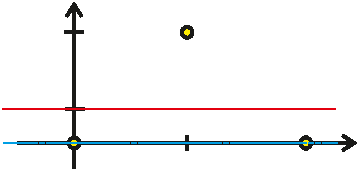
\includegraphics[width=13cm]{pictures/picture_1_F.pdf}};
    \draw [color=red](4.5,-0.2) node[anchor=north west] {LS line};
    \draw [color=blue](4.5,-1.3) node[anchor=north west] {MAD line};
    \draw [color=black](4.45,-2.5) node[anchor=north west] {$1$};
    \draw [color=black](0,-2.35) node[anchor=north west] {$\frac{1}{2}$};
    \draw [color=black](-4.55,1.8) node[anchor=north west] {$\frac{1}{2}$};
    \draw [color=black](-4.55,-1) node[anchor=north west] {$\frac{1}{6}$};
    \end{tikzpicture}
\end{center}

\begin{remark}
I když $ s^{2}_{n} $ je nestranný odhad $ \sigma^{2} $, $ s_{n} $ je vychýlený odhad $ \sigma $!
Je to obecná vlastnost odhadů (nestranných) rozptylů, neboť $ s^{2} $ nestranný odhad $ \sigma^{2} \, \Rightarrow \E[s] \leq \sigma $ 
\end{remark}


Uvažujme náhodnou veličinu $ X $  pro kterou platí, že $ \D [ X ] < + \infty $
\begin{equation*}
\begin{aligned}
 \E [X^{2}] = \D [ X ] +  \E [X]^{2} \quad \text{dosazením} \quad X = s \quad \text{dostaneme} \\
  \E [s^{2}] = \D [ s ] +  \E [s]^{2}
 \end{aligned} 
\end{equation*}
\begin{equation}
\E [s]^{2} \leq \sigma^{2} \quad \E [s] \leq \sigma
\end{equation}
a rovnost nastává pokud $ \D [ s ] = 0 $.

Například pro normální chyby je $ s_{n}^{2} \, \propto \, \chi^{2} \, \Rightarrow \, \E [s_{n}] < \sigma $

\begin{remark}
	předpokládali jsme, že hdnoty $ x_{i} $ jsou dány přesně, což nemusí být vždy pravda. Často obě veličiny $ (x,y) $ jsou měřeny nepřesně. EIV models "error in variable" v těchto modelech jsou často preferovány jiné odhady než LSE. Populární metoda: total least squares (ortogonal least squares). Zde minimalizujeme $ \sum_{i=1}^{n} d_{i}^{2} $, kde $ d_{i} $ je minimální vzdálenost bodu a přímky (kolmice na přímku protínající bod). To znamená, že neupřednostňujeme veličinu $ x $, ale přistupujeme k $ x $ a $ y $ rovnoměrně.
\end{remark}

\begin{center}    
    \begin{tikzpicture}
    \node[inner sep=0pt] (pic) at (0,0)
    {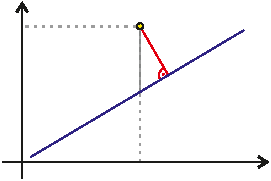
\includegraphics[width=13cm]{pictures/picture_2_F.pdf}};
    \draw [color=red](1.0,2.3) node[anchor=north west] {$d_{i}$};
    \draw [color=red](2.0,1.0) node[anchor=north west] {TLS vzdálenost};
    \draw [color=gray](-2.6,1.7) node[anchor=north west] {LS vzdálenost};
    \draw [color=red!20!black](0.0,3.80) node[anchor=north west] {$ (x_{i},y_{i}) $};
    \draw [color=black](5.45,-3.65) node[anchor=north west] {$x$};
    \draw [color=black](0,-3.65) node[anchor=north west] {$x_{i}$};
    \draw [color=black](-6.25,3.8) node[anchor=north west] {$y$};
    \draw [color=black](-6.25,3.3) node[anchor=north west] {$y_{i}$};
    \end{tikzpicture}
\end{center}

\begin{remark}
v literatuře se někdy $ x $ uvažují jako realizace náhodné veličiny ( ne vždy se $ x $ nastavuje předem, nebo je jasně dané (třeba pohlaví -- ???? (8 strana)) 
\end{remark}
Model má potom tvar
$$
 \E [ Y_{i} \vert X_{i} ] = \beta_{0} + \beta_{1} \quad  \D [ Y_{i} \vert X_{i} ] = \sigma^{2}
$$
pro většinu výsledků prezentovaných v této přednášce ale není podstatné, zde je $ x $ chápáno jako pevné nebo náhodné.
Důkazy většinou fungují s podmíněnými výrazy $ ( \E , \D , \dots )  $ při dané hodnotě $ x $ místo nepodmíněných.
Nicméně větší pozornost je třeba u odvození asymptotických rozdělení odhadů.

\subsection{Vlastnosti odhadů}
Vlastnosti odhadů $ \widehat{\beta}_{0} , \widehat{\beta}_{1} ,  s_{n}^{2} $.
\begin{theorem}
   Nechť $ \widehat{\beta}_{0} , \widehat{\beta}_{1} $ jsou $ \mathrm{LSE} $ odhady parametrů $ \beta_{0}, \beta_{1} $ v lineárním modelu 
   $$
   		Y_{i} = \beta_{0} + \beta_{1} x_{i} + e_{i} \quad i = 1 , \dots , n ,
   $$
   kde $ e_{i} $ jsou nezávislé náhodné veličiny (postačí i nekorelovanost) se stejným rozptylem $ \sigma^{2} $. Potom platí:
   \begin{enumerate}
  \item $ \E [ \widehat{\beta}_{0} ] = \beta_{0} \quad , \quad \E [ \widehat{\beta}_{1} ] = \beta_{1} $ , (nestranné odhady)
  \item $  \D [ \widehat{\beta}_{0} ] = \frac{\sigma^{2}}{S_{xx}}  \quad $ , kde $ \quad S_{xx} = \sumin (x_{i} - \oxnn )^{2} $
  \item $ \D [ \widehat{\beta}_{0} ] = \sigma^{2} \left( \frac{1}{n} + \frac{\oxnn ^{2}}{S_{xx}} \right) $
  \item Pokud navíc platí, že $ e_{i} \sim \NN ( 0 , \sigma^{2} ) \quad i = 1 , \dots , n \quad $ potom $ \quad \widehat{\beta}_{j} \sim \NN ( \beta_{j} , \D [ \widehat{\beta}_{j} ] ) \quad j = 0 , 1  $ 
\end{enumerate}
\end{theorem}
\begin{proofname}

   \begin{enumerate}
  \item upravíme $ \widehat{\beta}_{1} $
  		\begin{equation*}
  		\begin{aligned}
  		    \widehat{\beta}_{1} = \dfrac{\sum_{i=1}^{n} y_{i} x_{i} - n \overline{x}_{n} \overline{y}_{n}}{\sum_{i=1}^{n} x_{i}^{2} - n \overline{x}_{n}^{2}} = \frac{\sumin (x_i - \oxnn )(y_i - \oynn )}{\sumin (x_i - \oxnn )^{2}} = \\
  		    = \frac{1}{S_{xx}} \left( \sumin (x_i - \oxnn ) y_i - \oynn \sumin (x_i - \oxnn )  \right) =  \frac{1}{S_{xx}} \sumin (x_i - \oxnn ) y_i 
  		    \end{aligned}
  		\end{equation*}
  		potom má střední hodnota $ \widehat{\beta}_{1} $ tvar
  		\begin{equation*}
  		\begin{aligned}
  		    \E [ \widehat{\beta}_{1} ] = \E \left[ \frac{1}{S_{xx}} \sumin (x_i - \oxnn ) Y_i \right] = \frac{1}{S_{xx}} \sumin (x_i - \oxnn ) \E [ Y_i ] 
  		    = \frac{1}{S_{xx}} \sumin (x_i - \oxnn ) ( \beta_{0} + \beta_{1} x_i ) = \\ = \frac{\beta_{0}}{S_{xx}} \sumin (x_i - \oxnn ) + \frac{\beta_{1}}{S_{xx}} \sumin (x_i - \oxnn ) x_i = 0 + \frac{\beta_{1}}{S_{xx}} S_{xx} = \beta_{1}
  		    \end{aligned}
  		\end{equation*}
  		a střední hodnota pro $ \widehat{\beta}_{0} $ má tvar 
  		\begin{equation*}
  		\begin{aligned}
  		    \E [ \widehat{\beta}_{0} ] = \E [ \oyn - \widehat{\beta}_{1} \oxn ] = \E [ \oyn ] - \oxnn \E [ \widehat{\beta}_{1} ] = \dfrac{1}{n} \sumin \E [ Y_i ] - \oxnn \beta_1 = \beta_0 + \frac{\beta_1}{n} \sumin x_i - \oxnn \beta_1 = \beta_0
  		    \end{aligned}
  		\end{equation*}
  \item \begin{equation*}
  			\D [ \widehat{\beta}_{1} ] = \D \left[ \frac{1}{S_{xx}} \sumin (x_i - \oxnn ) Y_i \right] = \frac{1}{S_{xx} ^{2}} \sumin (x_i - \oxnn )^{2} \D [ Y_i ] = \frac{\sigma^{2} S_{xx}}{S_{xx}^{2}} = \frac{\sigma^{2}}{S_{xx}}
  		\end{equation*}
  \item  \begin{equation*}
  \begin{aligned}
  			\D [ \widehat{\beta}_{0} ] = \D [ \oyn - \widehat{\beta}_{1} \oxnn ] = \d [ \oyn ] + \oxnn ^{2} \D [ \widehat{\beta}_{1} ] - 2 \oxnn \text{cov}(\oyn , \widehat{\beta}_{1} ) = \\
  	= \frac{\sigma^{2}}{n} + \frac{\oxnn ^{2} \sigma^{2} }{S_{xx}} - 2 \oxnn \text{cov}( \oyn ,  \widehat{\beta}_{1} ) \\
\text{cov}( \oyn ,  \widehat{\beta}_{1} ) = \text{cov} \left( \oyn , \frac{1}{S_{xx}} \sumin ( x_i - \oxnn ) Y_i \right) = \frac{1}{S_{xx}} \sumin ( x_i - \oxnn ) \, \text{cov} ( \oyn , Y_i )  \\
\text{cov} ( \oyn , Y_i ) = \text{cov} ( \frac{1}{n} \sumjn Y_j , Y_i ) =  \frac{1}{n} \sumjn \text{cov} ( Y_j , Y_i ) = \frac{1}{n} \text{cov} ( Y_i , Y_i ) =  	\frac{1}{n} \D Y_i =  \frac{\sigma^{2}}{n}	\\
\Rightarrow  \text{cov}( \oyn ,  \widehat{\beta}_{1} ) = 0 = \frac{\sigma^{2}}{n S_{xx}} \sumin ( x_i - \oxnn )	
  			\end{aligned}
  		\end{equation*}
\end{enumerate}
\end{proofname}



